\chapter{The Conical Form as the 3D Envelope of the Spiral}\label{ch:cone}

\begin{figure}[t]
  \centering
  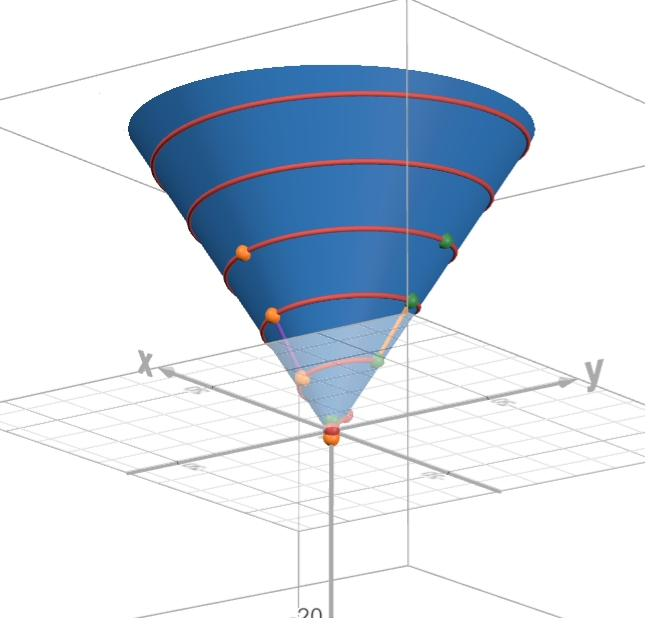
\includegraphics[width=0.72\textwidth]{bilder/Helix_3d}
  \caption{The conical helix: the red spiral curve winds upward along the blue
    cone surface $z = -\tfrac{3}{4} + \tfrac{\pi}{2}\,r$. The orange points
    mark the integer values $k(n)$ at $n \equiv 1 \pmod{6}$, and the green
    points the values at $n \equiv 5 \pmod{6}$. The apex of the cone is
    located at $P_0 = (0,\,0,\,-\tfrac{3}{4})$; the light triangle in the
    foreground shows the radial cross-section and illustrates the constant
    slope $\Delta z / \Delta r = \pi/2$ of the generatrix.}
  \label{fig:conical-helix-main}
\end{figure}

\section{From the 2D Model to the Conical Form}

The spiral investigated previously possesses a pronounced arithmetic structure:
the points $P_n$ lie on radii whose distances are determined by the quadratic
sequence
\[
k(n) = \frac{2n^2 + 3n + 1}{6}.
\]
Particularly distinguished are the values
\[
n \equiv 1,5 \pmod{6},
\]
for which the mean values $k(n)$ are integers. These two classes form an
alternating ray system that repeats every six steps.

The observation that these rays exhibit a regular structure in the plane
naturally leads to the question of whether there exists a three-dimensional
form that geometrically bundles this structure. The answer is a cone: it
forms an envelope in which the alternating rays appear as lines on the
surface and the spiral itself can be interpreted as a space curve on this
surface.

\section{The 3D Form as a Cone of Revolution}

The three-dimensional structure arises from a geometrically unique process.
The starting point is the two-dimensional term curve
\[
r = r(p), \qquad \varphi = \varphi(p),
\]
whose path we cut along the vertical axis. If this curve segment is erected
perpendicular to the plane and then wound spirally about the $z$-axis along
its length, the resulting three-dimensional surface has a straight generatrix
--- a \emph{cone of revolution}.

This can be justified as follows:

\begin{itemize}
  \item The radial increments of the sequence are constant:
  \[
  \Delta r = \frac{12}{\pi}.
  \]
  A surface on which equal radial increments lie along a fixed direction is
  necessarily a conical surface.

  \item The sequence possesses a periodic structure with
  \[
  \Delta n = 6.
  \]
  This periodicity is translated into a constant slope along the height when
  the curve is wound up.

  \item When a planar curve with constant radial increment is wound up, the
  resulting surface has a straight generatrix. This is precisely the defining
  property of a cone.
\end{itemize}

Thus the three-dimensional form is a direct geometric consequence of winding
up the 2D curve. The spiral that arises on this surface is therefore a
\emph{conical helix}, and the cone itself is the natural envelope of the
original two-dimensional structure.

\section{Radial Structure and 6-Periodicity}

Between two rays of the same class (i.e.\ two values of $n$ with
$n \equiv 1 \pmod{6}$ or two values with $n \equiv 5 \pmod{6}$) there is
always
\[
\Delta n = 6.
\]

The corresponding radial increment of the spiral is
\[
\Delta r = \frac{12}{\pi}.
\]

These two values form the basis of the cone geometry: they determine the
slope of the cone and hence its opening angle.

\section{Derivation of the Cone Slope}

We consider the cross-section of the cone with a plane through the axis of
revolution. This yields a right triangle with
\[
\text{horizontal leg: } \Delta r = \frac{12}{\pi}, \qquad
\text{vertical leg: } \Delta z = 6.
\]

The slope of the cone is given by
\[
\frac{\Delta z}{\Delta r}
= \frac{6}{12/\pi}
= \frac{\pi}{2}.
\]

Thus the generatrix of the cone has the equation
\[
z = \frac{\pi}{2}\,r + b
\]
in the $(r,z)$-cross-section.

\section{The Vertex of the Quadratic Sequence as the Cone Apex}

The constant $b$ follows directly from the structure of the quadratic
sequence. The vertex of the parabola
\[
k(n) = \frac{2n^2 + 3n + 1}{6}
\]
is located at
\[
n_0 = -\frac{3}{4}.
\]

This value marks the natural origin of the construction: it is the point of
minimal slope of the sequence and hence the geometric starting point of the
cone projection.

We identify
\[
z_0 = n_0 = -\frac{3}{4}, \qquad r_0 = 0.
\]

The point $(0,-\tfrac{3}{4})$ must therefore lie on the cone. Substituting
into the cone equation yields
\[
-\frac{3}{4} = \frac{\pi}{2}\cdot 0 + b,
\]
hence
\[
b = -\frac{3}{4}.
\]

The final cone equation is therefore:
\[
\boxed{
z = -\frac{3}{4} + \frac{\pi}{2}\,r
}
\]

\section{Cone Surface and Generatrix}

The cone surface is the set of all points $(r,\varphi,z)$ satisfying the
linear relationship between radius and height:
\[
z(r) = -\frac{3}{4} + \frac{\pi}{2}\,r.
\]

Each line on the surface corresponds to a fixed angular direction $\varphi$.
The alternating rays of the sequence lie exactly on such generatrices.
Their 6-periodicity is encoded by the constant slope of the cone.

\section{Verification: The Conical Helix Lies Entirely on the Cone Surface}

\begin{theorem}[Helix Lies on the Cone]\label{thm:helix-on-cone}
The conical helix defined in Chapter~\ref{ch:helix},
\[
\gamma(\theta)
= \Bigl(\tfrac{6}{\pi^2}\theta\cos\theta,\;
        \tfrac{6}{\pi^2}\theta\sin\theta,\;
        -\tfrac{3}{4}+\tfrac{3}{\pi}\theta\Bigr),
\]
lies entirely on the cone surface
$z = -\tfrac{3}{4} + \tfrac{\pi}{2}\,r$ for all $\theta \geq 0$.
\end{theorem}

\begin{proof}
We must show that the $z$-coordinate of the helix equals
$-\tfrac{3}{4} + \tfrac{\pi}{2}\,r(\theta)$. We have:
\[
  r(\theta) = \frac{6}{\pi^2}\,\theta,
\]
and therefore
\[
  -\frac{3}{4} + \frac{\pi}{2}\,r(\theta)
  = -\frac{3}{4} + \frac{\pi}{2}\cdot\frac{6}{\pi^2}\,\theta
  = -\frac{3}{4} + \frac{3}{\pi}\,\theta
  = z(\theta). \qedhere
\]
\end{proof}

\begin{remark}\label{rem:algebraic-core}
The identity $\frac{\pi}{2}\cdot\frac{6}{\pi^2} = \frac{3}{\pi}$ is the
algebraic core of the entire 3D model: the cone slope $\frac{\pi}{2}$ and
the spiral parameter $a = \frac{6}{\pi^2}$ are exactly matched so as to
produce the height function $z = \frac{3}{\pi}\theta$. This relationship
follows from the choice $\Delta z = 6$ and $\Delta r = \frac{12}{\pi}$,
since
\[
  \frac{\Delta z}{\Delta r} = \frac{6}{12/\pi} = \frac{\pi}{2}
  \qquad\text{and}\qquad
  \frac{\pi}{2}\cdot a = \frac{\pi}{2}\cdot\frac{6}{\pi^2} = \frac{3}{\pi}.
\]
In Chapter~\ref{sec:visualisierung} this cone conformity is verified purely
algebraically via the universal quantity $Q(k) = \sqrt{48k+1}$
(Theorem~\ref{satz:kegel}).
\end{remark}
